% Articolo formato A4 con carattere 11pt
\documentclass[a4paper,11pt]{article}

% Listing di programmi
\usepackage{verbatim}
% Caricamente codec UTF8
\usepackage[utf8]{inputenc}
% lingua ita, serve anche per far comparire la scritta "Riferimenti Bibliografici" in italiano
\usepackage[italian]{babel}
\usepackage{listings}
% cambio i margini
\usepackage{vmargin}
\setpapersize{A4}
\setmarginsrb{25mm}{0mm}{25mm}{5mm}%
             {0mm}{10mm}{0mm}{10mm}

% Per l'inserimento delle immagini
\usepackage{graphicx}

% Setta alcuni attributi del titolo
\title{Implementazione Algoritmo di Chiusura di Congruenza Nelson-Oppen}
\author{Federico De Meo VR355974}

\begin{document}

% Stampa titolo
\maketitle

\footnotesize
% L'asterisco evita che compaia il numero a fianco del titolo
\section*{Introduzione}
Questo documento descrive l'implementazione della procedura di Nelson-Oppen \cite{congruenclosure}, descritta a lezione, per il calcolo della soddisfacibilità di formule scritte nell'unione delle segnature della teoria dell'uguaglianza e di quella delle liste. Oltre alla semplice implementazione dell'algoritmo proposto dal libro sono state introdotte delle euristiche che hanno portato a notevoli migliorie prestazionali che saranno esaminate nel seguito.
Il linguaggio di programmazione scelto è Java, il quale offre un variegato insieme di strutture dati molto utili e ben implementate.
Si farà anche un confronto con l'algoritmo proposto da Downey, Sethi e Tarjan\cite{downey-sethi-tarjan-1980} implementato da Marco Tamassia.

\section{Parser}
L'implementazione del progetto inizia con la stesura del parser, il cui scopo è quello di leggere le formule nelle due teoria dell'uguaglianza $(T_E)$ e delle liste $(T_{cons})$.
Per fare ciò si è scelto di utilizzare il compilatore \emph{JavaCC} \cite{javacc} il quale, definita una grammatica context-free BNF, genera le classi necessarie per il riconoscimento delle formule in input.
La peculiarità di \emph{JavaCC} è quella di generare sia un analizzatore lessicale sia uno sintattico, partendo semplicemente dal file della grammatica.

La grammatica scelta che descrive la sintassi delle formule accettate è la seguente:
\begin{verbatim}
Formula ::= Clausola (& Clausola)*
Clausola ::= Token = Token | Token != Token | atom(Token) | !atom(Token)
Token ::= cons(Token,Token) | car(Token) | cdr(Token)  | Fun(Token(,Token)*) | [a-z]+[0-9]*
Fun ::= [A-Z][a-z0-9]*
\end{verbatim}
Come riportato dal testo, ci concentreremo solo sul frammento senza quantificatori.
Questa grammatica è stata riportata nel file {\tt grammar.jj} al quale è stato aggiunto codice Java che definisce la semantica per la costruzione del DAG su cui opera l'algoritmo.
Inoltre si è scelto di generare un errore qualora nella formula vi siano due funzioni con stesso nome e diversa arietà.
\section{Scelte implementative}
Oltre alla possibilità di utilizzare il programma tramite riga di comando si è scelto di implementare una piccola interfaccia grafica al fine di agevolare l'uso dell'applicazione.
La classe principale, {\tt verifica/Main.java}, avvia l'una o l'altra modalità.
Nello stesso file è stato anche implementato l'algoritmo, oggetto di questo documento, in due versioni: "semplice" e con euristiche.
Per separare le due implementazioni si è scelto di riscrivere due volte ogni metodo differenziando la loro segnatura.
In particolare la segnatura prevede che:
\begin{itemize}
	\item i metodi che fanno parte dell'implementazione con euristiche terminino tutti con il carattere H (e.g.: mergeH(...));
	\item i metodi che fanno parte dell'implementazione semplice inizino tutti con il carattere \_ (e.d.: \_merge(...)).
\end{itemize}
L'avvio dell'algoritmo di chiusura di congruenza è dato dall'invocazione del metodo  
{\tt execCC(String formula, JResult window)}
dove {\tt formula} è la formula di cui verificare la soddisfacibilità e {\tt window} è un oggetto {\tt JResult} che rappresenta la finestra che visualizzerà l'output dell'algoritmo (parametro usato solo nell'invocazione con GUI).
\subsection{Strutture dati di supporto}
Nella prima fase di esecuzione viene chiamato il parser, al quale vengono passate, oltre alla stringa in input, diverse strutture dati di supporto:
\begin{itemize}
	\item \emph{Graph}: {\tt HashMap} che mantiene la struttura del grafo;
	\item \emph{equals}: {\tt ArrayList} che mantiene i nodi dei letterali uguali;
	\item \emph{noEquals}: {\tt ArrayList} che mantiene i nodi dei letterali diversi;
	\item \emph{consList}: {\tt ArrayList} che mantiene i nodi dei {\tt car()} e {\tt cdr()} degli operatori {\tt cons()} di cui fare la prima serie di {\tt MERGE};
	\item \emph{atoms}: {\tt ArrayList} che mantiene i nodi {\tt atom()};
	\item \emph{consfn}: {\tt ArrayList} che mantiene i nodi {\tt cons()} che NON dovranno apparire in \emph{atoms}.
\end{itemize}
Si noti una particolarità: le strutture \emph{equals}, \emph{noEquals} e \emph{consList} rappresentano logicamente coppie di nodi che devono essere usate per effettuare le {\tt MERGE}.
La struttura {\tt ArrayList}, però, non gestisce coppie bensì singoli elementi in successione.
Si è ugualmente scelta questa struttura avendo cura di riempirla in modo che un elemento in posizione pari sia in relazione con il successivo elemento in posizione dispari. $(2i \sim 2i+1)$
\subsection{Gestione dei nodi}
In ogni struttura dati usata dall'algoritmo si è deciso di memorizzare un oggetto {\tt Node} in modo tale da avere direttamente il riferimento al nodo.
Si noti che questa scelta è stata preferita a quella di utilizzare delle chiavi, in quanto, a seguito di diversi test, la gestione delle chiavi, seppure tramite strutture Hash, comportava un considerevole aumento dei tempi di computazione.
\subsection{Algoritmo}
Dopo la fase di parsing viene chiamato uno dei due metodi {\tt NelsonOppenSpeedUp()} o {\tt NelsonOppen()} che rispettivamente eseguono l'algoritmo con e senza euristiche.
Non mi soffermerò sulla specifica dell'algoritmo privo di euristiche in quanto ampiamente descritto sul testo di riferimento nel Capitolo 9 (pag. 251-258).

\subsection{Euristiche}
Al fine di migliorare le prestazioni dell'algoritmo di Nelson-Oppen, sono state introdotte diverse euristiche qui riportate in dettaglio:

\begin{itemize}
	\item {\bf Compressione dei cammini\cite{cormen}:} l'algoritmo di Nelson-Oppen utilizza gli insiemi disgiunti per rappresentare le classi di congruenza che dovranno essere unite. Ogni elemento di un insieme disgiunto ha un campo {\tt find} che lo unisce in catena al rappresentante della classe a cui appartiene.
La compressione dei cammini è un'euristica che collega direttamente ogni nodo con il rappresentante della classe.
Per fare ciò, ogniqualvolta viene chiamato il metodo {\tt find(id)}, vengono modificati tutti i campi {\tt find} dei nodi visitati, aggiornandoli con l'id del rappresentante.
	\item {\bf Unione per rango \cite{cormen}:} anche questa euristica migliora la struttura per insiemi disgiunti.
In particolare definisce un criterio con il quale scegliere il nuovo rappresentante in fase di {\tt union}, criterio non definito nell'algoritmo riportato sul testo dove la scelta è arbitraria.
Con l'unione per rango viene scelto come nuovo rappresentante la radice del sottoalbero con più nodi, a cui unire la radice del sottoalbero con meno nodi. Per semplificare il mantenimento del numero di nodi di ogni sottoalbero è stato introdotto un campo {\tt rank} nell'oggetto {\tt Node}.
Il {\tt rank} serve a mantenere un limite superiore all'altezza del nodo stesso, la radice con il rango più piccolo viene fatta puntare alla radice con rango maggiore.
Così facendo un minor numero di nodi, con lunghe catene di find, saranno visitati prima di raggiungere il nuovo rappresentante. 
	\item {\bf Letterali vietati:} quest'ultima euristica non riguarda gli insiemi disgiunti ma aiuta a terminare la computazione di una formula non soddisfacibile appena si scopre una contraddizione.
L'idea è quella di controllare se, in fase di {\tt merge}, le due classi unite non diano origine ad una incongruenza.
Per fare questo ogni {\tt Node} è stato arricchito con una struttura {\tt HashSet} che mantiene l'insieme dei termini proibiti (da adesso $forbidden$) per quel nodo.
La lista viene arricchita in fase di parsing: ogniqualvolta si incontra una disuguaglianza
$F: ... s_{m} \not= t_{m} ... $, viene arricchito l'insieme $forbidden$ di $s_{m}$ aggiungendo $t_{m}$ e analogamente ai $forbidden$ di $t_{m}$ si aggiunge $s_{m}$.
Restano quindi da fare alcuni semplici controlli prima di consentire una {\tt merge(id1,id2)}.
Il primo controllo verifica che nei $forbidden$ del rappresentante di {\tt id1} non sia presente il nodo {\tt id2}.
Vista la natura della struttura dati {\tt HashSet} questo controllo viene fatto in tempo atteso $O(1)$.
Gli altri due controlli verificano in quale classe di congruenza si trovano i $forbidden$ di {\tt id1} e di {\tt id2}.
In particolare, se il rappresentante di un $forbidden$ di {\tt id1} è uguale al rappresentante di {\tt id2} (e viceversa), allora le due classi non devono essere unite e l'algoritmo termina restituendo insoddisfacibile.
Altrimenti si procede con la fase di unione e l'insieme $forbidden$ viene propagato al nuovo rappresentante, mantenendo la struttura aggiornata.
\end{itemize}
Le prime due euristiche sono applicabili al caso generale di formula soddisfacibile o non soddisfacibile, migliorando molto l'algoritmo semplice di Nelson-Oppen.
L'ultima euristica aiuta solo in caso di formula insoddisfacibile, abbattendo il tempo di computazione e portandolo sotto all'implementazione di Downey, Sethi e Tarjan la quale non si presta a questo genere di euristica.
\subsection{Generatore di formule}
Al fine di generare benchmark considerevoli, si è implementato un piccolo generatore di formule casuali.
Questo generatore è accessibile solo dall'interfaccia grafica e consente di generare una qualsiasi formula casuale accettando come paramentri: numero di uguaglianze, disuguaglianze, atomi e non atomi.
La probabilità di generare formule insoddisfacibili è molto alta, ma specificando solo clausole di uguaglianza è possibile generare formule soddisfacibili.
\section{Test}
Nel seguito sono riportati i risultati dei test effettuati sulle medesime formule con le tre diverse implementazioni: Nelson-Oppen (NO), Nelson-Oppen con euristiche (NO+) e Downey, Sethi e Tarjan (DST) quest'ultimo implementato da Marco Tamassia.

I test sono stati effettuati su una macchina avente processore i7 a 2,4GHz con sistema operativo Ubuntu 11.04 e JVM v1.6.0 prodotta da Sun/Oracle.
Nell'allegata cartella TEST è presente un sottoinsieme delle formule usate. Questo perché, essendo stati generati molti test per meglio studiare le performance delle tre implementazioni, le dimensioni dell'allegato sarebbero state improponibili.
Si è adoperato uno script, anch'esso in allegato, per l'esecuzione automatizzata di test prestazionali.

\begin{table}[htp]
\caption{Prestazioni su problemi di varie dimensioni (clausole miste)}
\centering
\begin{tabular}{| l | l | l | l | l | l |}
\hline
Risultato & Nodi & Archi & DST (ms) & NO + eur (ms) & NO (ms) \\
\hline
Insoddisfacibile & 1039 & 1668 & 159 & 111 & 348 \\
Insoddisfacibile & 2066 & 3452 & 232 & 449 & 3182 \\
Insoddisfacibile & 2793 & 4549 & 314 & 508 & 5396 \\
Insoddisfacibile & 3008 & 5341 & 346 & 523 & 6452 \\
Insoddisfacibile & 4853 & 7924 & 475 & 904 & 38843 \\
Insoddisfacibile & 6253 & 12538 & 663 & 1841 & 46955 \\
\hline
\end{tabular}
\end{table}

\begin{figure}[htp]
\caption{Andamento prestazioni con formule composte di clausole miste}
\centering
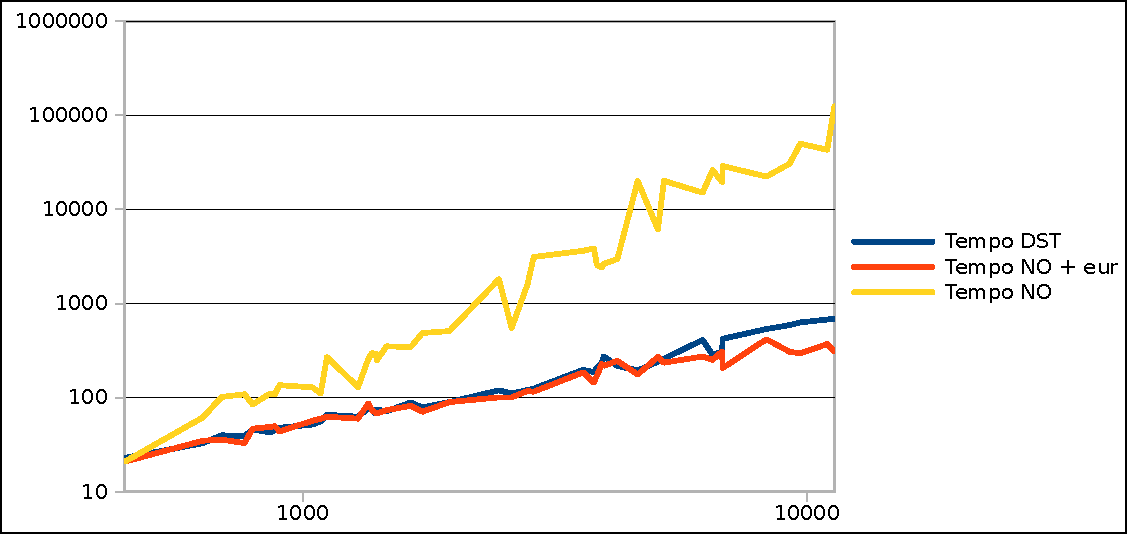
\includegraphics[scale=0.8]{mixed.pdf}
\end{figure}
\begin{table}[htp]
\caption{Prestazioni su problemi di varie dimensioni (clausole di sola equivalenza)}
\centering
\begin{tabular}{| l | l | l | l | l | l |}
\hline
Risultato & Nodi & Archi & DST (ms) & NO + eur (ms) & NO (ms) \\
\hline
Soddisfacibile & 486 & 664 & 103 & 39 & 105 \\
Soddisfacibile & 678 & 1003 & 128 & 66 & 205 \\
Soddisfacibile & 1029 & 1394 & 142 & 81 & 392 \\
Soddisfacibile & 1610 & 2299 & 179 & 114 & 1285 \\
Soddisfacibile & 2494 & 3809 & 261 & 266 & 4076 \\
Soddisfacibile & 3938 & 5509 & 330 & 289 & 18140 \\
Soddisfacibile & 5246 & 8991 & 456 & 421 & 37526 \\
\hline
\end{tabular}
\end{table}
\begin{figure}[htp]
\caption{Andamento prestazioni con formule composte di clausole di sola equivalenza}
\centering
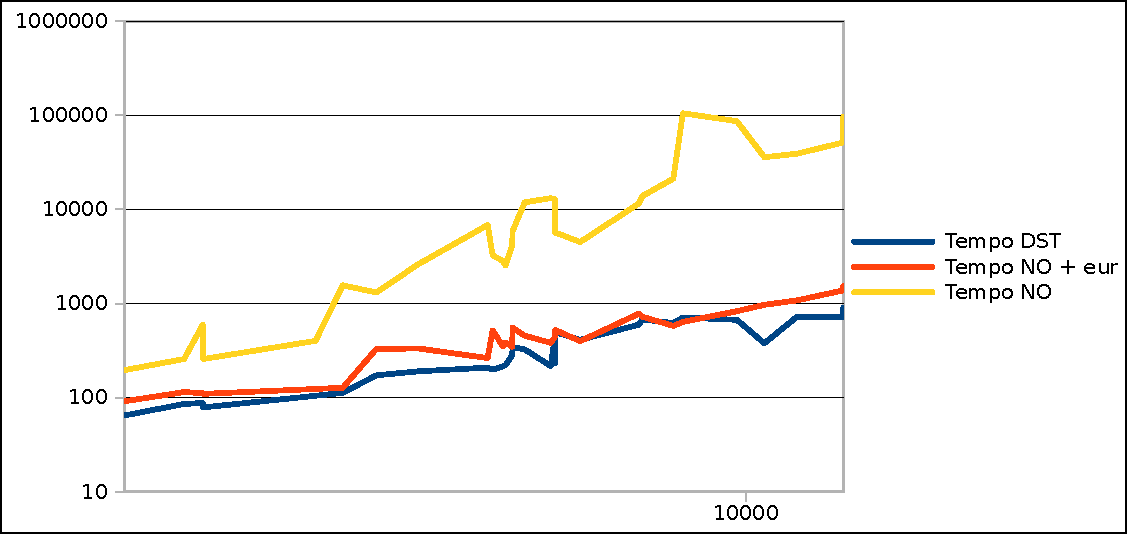
\includegraphics[scale=0.8]{eqonly.pdf}
\end{figure}

\par\bigskip
\par\bigskip\par\bigskip
\par\bigskip

\par\bigskip
\par\bigskip
\par\bigskip
\par\bigskip
\par\bigskip
\par\bigskip\par\bigskip
\par\bigskip\par\bigskip
\par\bigskip

\par\bigskip
\par\bigskip
\par\bigskip
\par\bigskip
\par\bigskip
\par\bigskip

\section{Considerazioni e conclusioni}
L'algoritmo di base NO presenta un andamento particolarmente altalenante.
La versione con euristiche ha portato ad una stabilità quasi inaspettata trattandosi di migliorie che non abbassano il grado di complessità dell'algoritmo di partenza.
L'algoritmo DST presenta invece una maggior stabilità in tutti i test, grazie alla sua complessità $O(e*\log(e)$.
In conclusione l'euristica dei nodi vietati su NO consente, talune volte, di terminare prima di DST ma a conti fatti il tempo risparmiato non è sufficiente da renderlo un'alternativa a DST.


\begin{thebibliography}{1}
\bibitem{congruenclosure}
Aaron R. Bradley, Zohar Manna - Springer - \textit {The calculus of computation} Capitolo 9
\bibitem{downey-sethi-tarjan-1980}
P. J. Downey, R. Sethi, R. E. Tarjan - Variations on the common subexpression problem - 1980
\bibitem{javacc}
T. Norvell - JavaCC tutorial - www.engr.mun.ca/$\sim$theo/JavaCC-Tutorial/javacc-tutorial.pdf
\bibitem{cormen}
Thomas H. Cormen, Charles E. Leiserson, Ronald L. Rivest, Clifford Stein - McGraw-Hill - \textit {Introduzione agli algoritmi e alle strutture dati}, Strutture dati per insiemi disgiunti, pagine 427-236
\bibitem{cyrluk-lincoln-shankar-1996}
D. Cyrluk, P. Lincoln, N. Shankar - On Shostak's decision procedure for combinations of theories - 1996
\bibitem{nieuweinhuis-oliveras-}
R. Nieuwenhuis, A. Oliveras - Fast congruence closure and extensions - 2007

\end{thebibliography}

\end{document}